\section{Struktur}

\begin{figure}[H]
	\center
	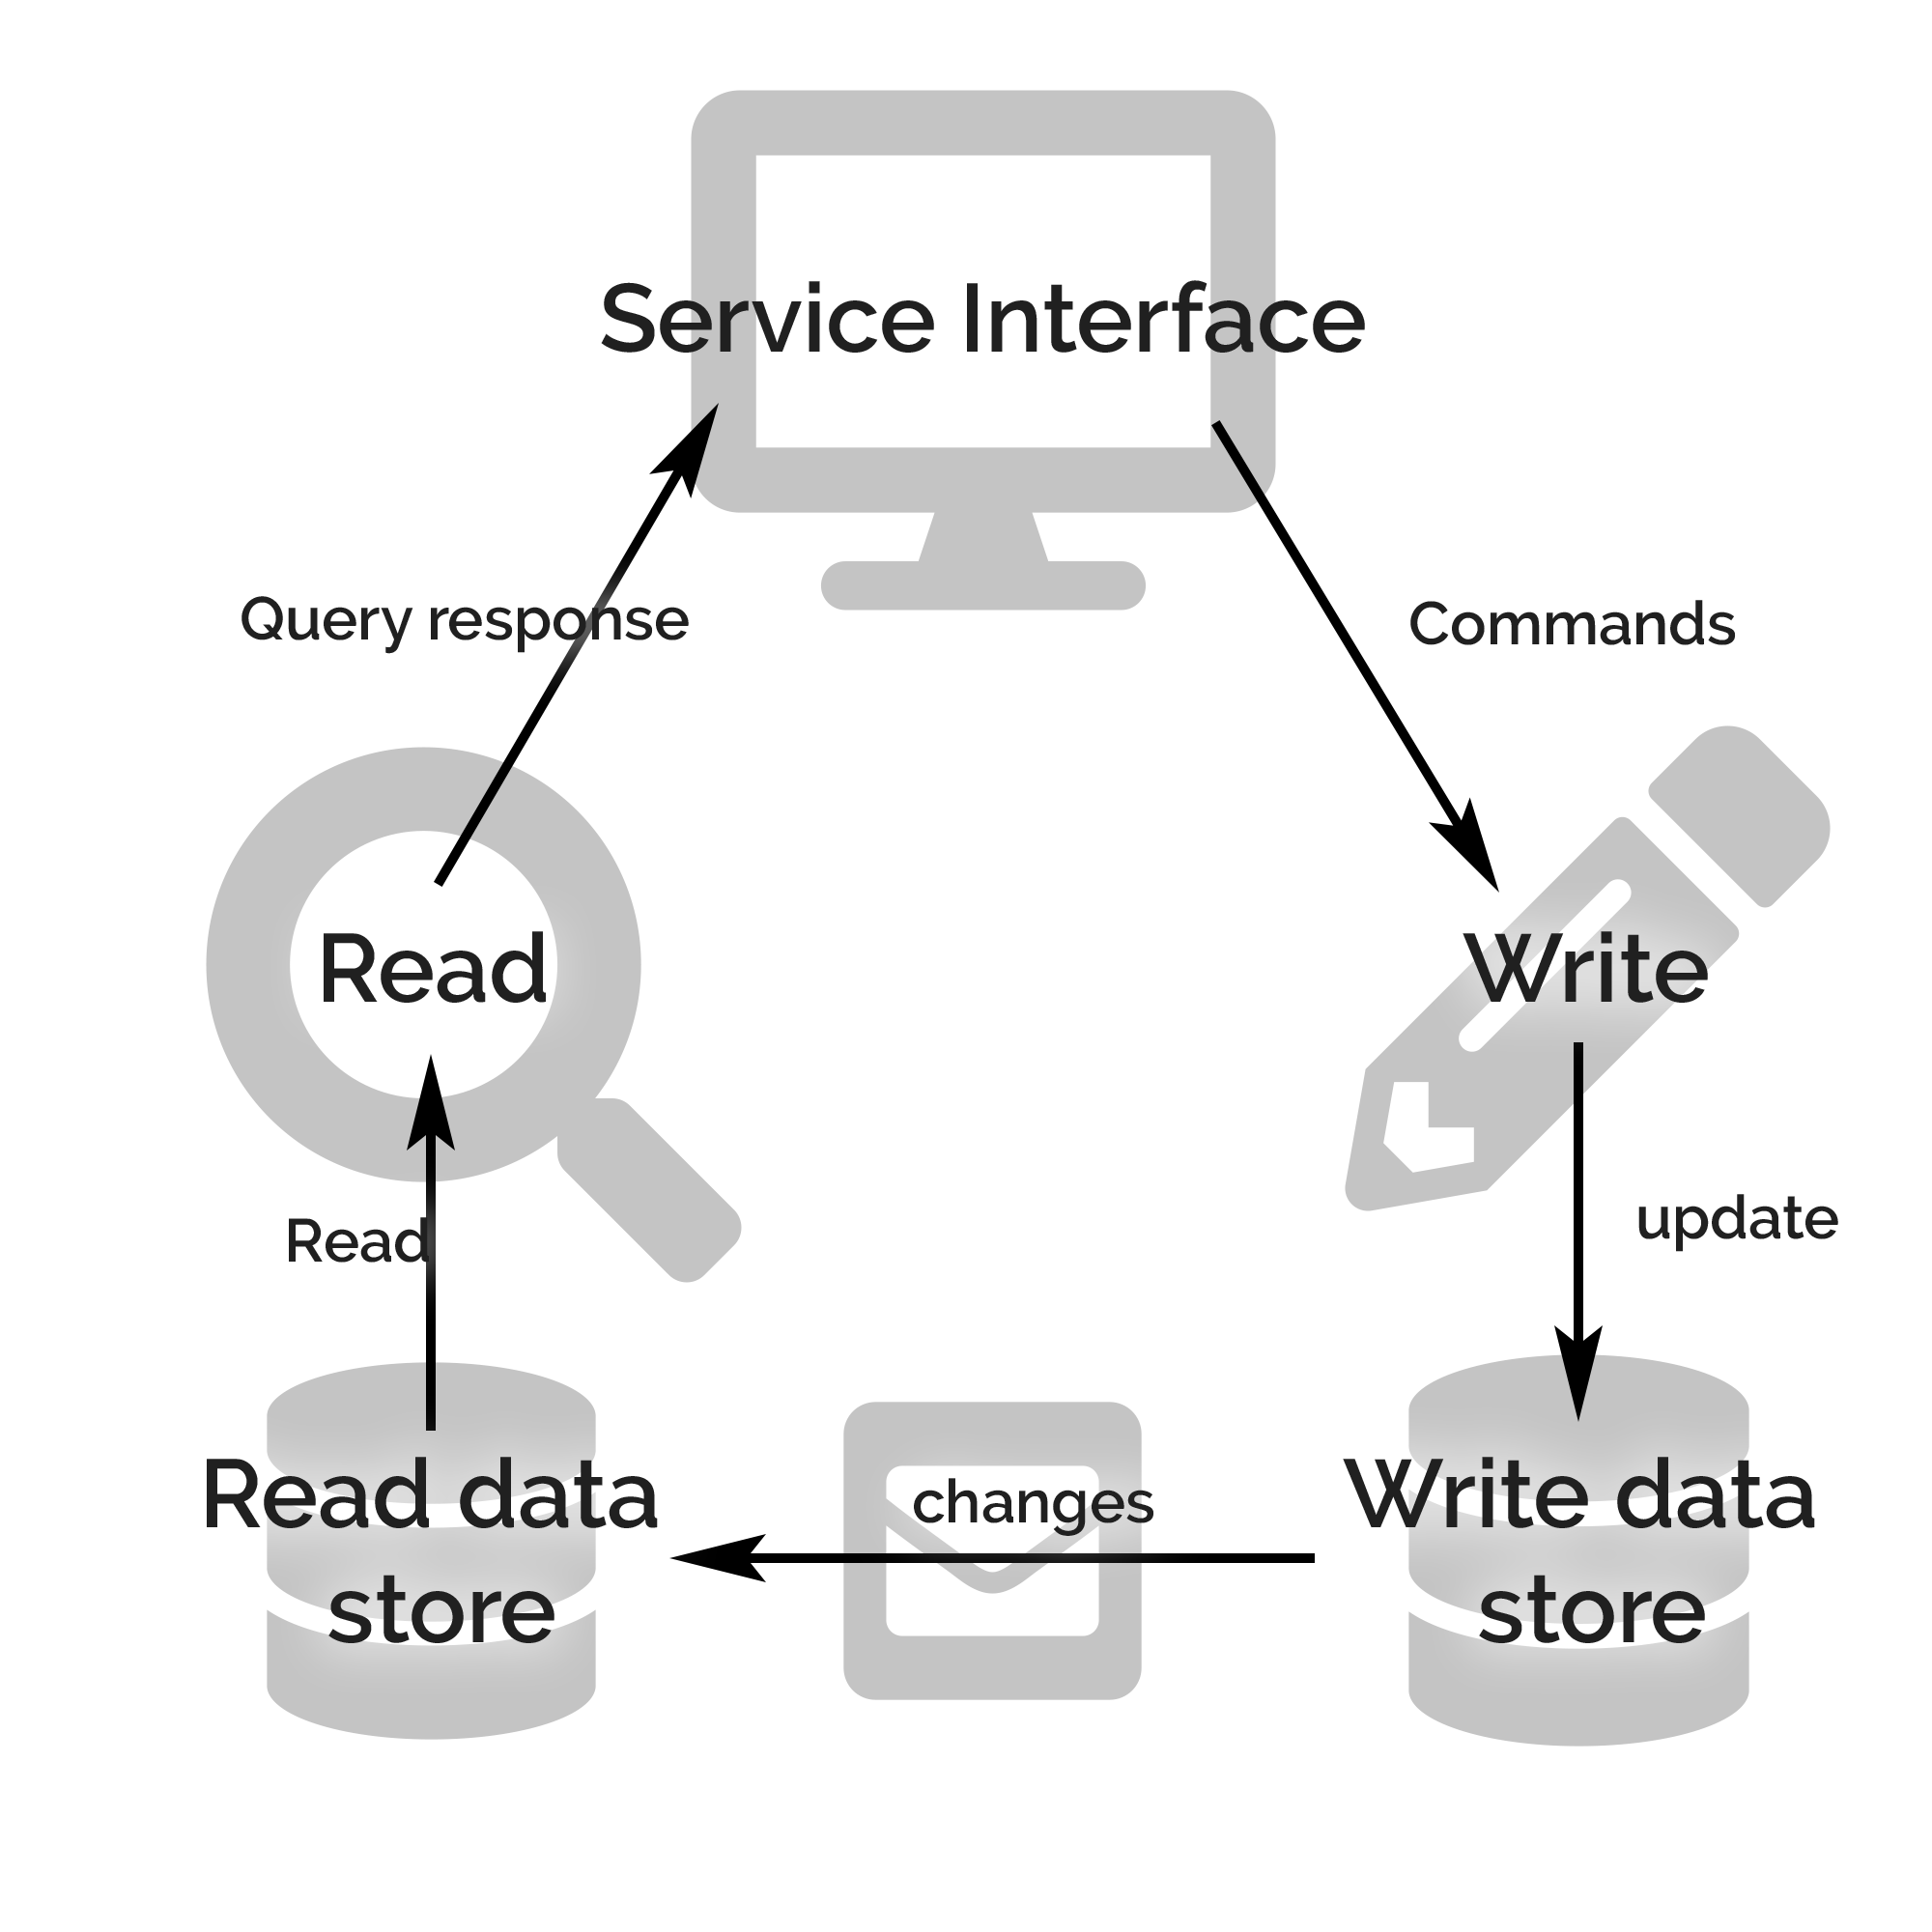
\includegraphics[width=0.5\textwidth]{CQRS-Model.png}
	\caption{Simpel CQRS med Read og Write}
	\label{fig:cqrs-model}
\end{figure}

Dette pattern består af 2 vitale dele, Read siden og Write siden, Disse 2 dele, gør at patternet effektivt kan skrive eller læse til en data store. Princippet er at disse dele er Rent (Pure) altså kun gør det som den er sat til. Write siden skriver kun til Datastore og returnere ikke nogen form for tilstand tilbage. Read siden ændre ikke data, men returnere kun Data. Disse handlinger er gjort igennem Commands og Queries.

\subsection{Generelt}

\begin{figure}[H]
	\center
	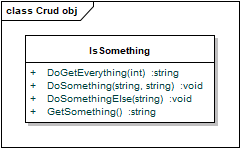
\includegraphics[width=0.3\textwidth]{class-one.png}
	\caption{Crud klasse}
	\label{fig:class-one}
\end{figure}

Et normalt objekt indeholder både Read og Write operationer, og nogle gange kombineret, se figur \ref{fig:class-one}.

\textit{``CQRS is simply the creation of two objects where there was previously only one. The separation occurs based upon whether the methods are a command or a query'' - Greg Young}

\begin{figure}[H]
	\center
	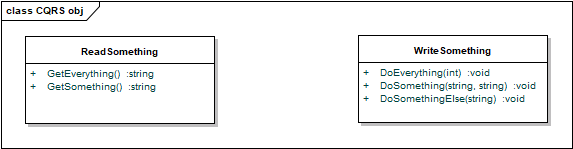
\includegraphics[width=0.7\textwidth]{class-two.png}
	\caption{CQRS klasse}
	\label{fig:class-two}
\end{figure}

Generelt består CQRS af Commands (WriteSomething) og Query reponses (ReadSomething) samt Events, se figur \ref{fig:class-two}. Commands rejser events når de bliver oprettet, og gør det muligt at opdatere Read siden. Denne opdeling gør det muligt, at udvikle disse sider totalt separeret, bortset fra den event bus, der binder det hele sammen.

Et scenarie der kan opstå er: Service interface sender en Command, til at ændre en model f.eks. oprette, slette, redigere en model, dette Command bliver valideret og bliver først persisteret på Write data store, men bliver også sendt til Read data store. Read data store bliver nu opdateret med frisk data, og nu opdateret med Write data store. I en anden instans kan Service interface anmode Read siden, med et query om en model fra Read data, og ønske at modtage et stykke data. Read siden opretter nu en DTO (Data Transfer Objects), og returnere den med det ønskede data.
\subsection{Read}

Read siden består Queries, hvor andre modeller kan anmode om DTO'er dette gør det let at hente data, næsten direkte fra Read data store, som næsten altid er opdateret af Write siden. Read data store, opfylder dog ikke \textit{Consistency} princippet, men nærmere \textit{Eventually Consistent} som gør at systemet skal tage højde for at der kan være samhørighedsproblemer på dataen. 
\subsection{Write}

Write siden består af Commands som kan ændre de modeller som findes i domain modellerne. Write siden opdatere sin egen data store, samt Read data store.
